%% Journal of Systems and Software — Elsevier CAS double-column template (v2.4)
%%
%% Every quantitative claim in this manuscript is traceable to a file listed in
%% paper/FACTS.md, which is generated by scripts/17_build_facts.py from
%% results/tables/*.csv. Numbers are not edited by hand here; if a number
%% changes, it is regenerated and the sentence quoting it is updated.

\documentclass[a4paper,fleqn]{cas-dc}

%% The CAS bundle references e-mail and social-media thumbnail images that are
%% not shipped with it, and raises a missing-file error for each. The class
%% declares \g_stm_nologo_bool to guard those includes but never sets it, and
%% offers no document option for it, so we set it here. This must come after
%% \documentclass, which is where cas-common.sty defines the boolean.
\ExplSyntaxOn
\bool_gset_true:N \g_stm_nologo_bool
\ExplSyntaxOff

\usepackage[authoryear,longnamesfirst]{natbib}
\usepackage{booktabs}
\usepackage{graphicx}
\usepackage{amsmath}
\usepackage{totpages}

%% The CAS class computes its own \lastpage at \AtEndDocument, before deferred
%% floats are flushed, so figures that land on trailing float pages are never
%% counted and the footer prints values like "Page 13 of 12". totpages counts
%% the pages actually shipped, which is what the footer means. The override has
%% to happen at \AtBeginDocument, because the class's value arrives in the .aux
%% file, which is read after this preamble.
\AtBeginDocument{\renewcommand{\lastpage}{\ref{TotPages}}}
\usepackage{float}
\graphicspath{{../figures/}}

%% Float placement. With the default limits, a dense two-column body pushes
%% every figure to the end of the document, because no page has enough legal
%% float area. Relaxing the fractions lets a figure sit near the text that
%% references it, which is what the journal asks for.
\renewcommand{\topfraction}{0.9}
\renewcommand{\bottomfraction}{0.8}
\renewcommand{\textfraction}{0.07}
\renewcommand{\floatpagefraction}{0.7}
\renewcommand{\dbltopfraction}{0.9}
\renewcommand{\dblfloatpagefraction}{0.7}
\setcounter{topnumber}{3}
\setcounter{bottomnumber}{2}
\setcounter{totalnumber}{4}
\setcounter{dbltopnumber}{2}

\begin{document}
\let\WriteBookmarks\relax
\def\floatpagepagefraction{1}
\def\textpagefraction{.001}

\shorttitle{The MCP server ecosystem}
\shortauthors{J. Chen}

\title[mode=title]{The Model Context Protocol Server Ecosystem:
An Empirical Study of Quality, Security, and Evolution}

\author[1]{Junan Chen}
\cormark[1]
\ead{chenjunan.aiden@gmail.com}
\credit{Conceptualization, Methodology, Software, Validation, Formal analysis,
Investigation, Data curation, Writing -- original draft, Visualization}

\affiliation[1]{organization={University of Electronic Science and Technology of China},
                city={Chengdu},
                state={Sichuan},
                country={China}}

\cortext[1]{Corresponding author.}

\begin{abstract}
AI agents reach external tools through the Model Context Protocol (MCP), and
the official registry publishes every server version with registry-side
timestamps, making a population-level study possible for the first time. We
analysed a complete snapshot frozen on 24 September 2026: 114,604 published
versions across 35,388 servers and 20,540 namespaces, enriched with package
metadata for 13,316 packages, tool definitions extracted from 1,200 package
sources, and repository data for 924 repositories. We established extraction
quality against human coding of 150 packages (recall 99.7\%, precision 99.7\%),
and two coders classified interface and security properties over 150 servers
and 200 tool definitions. Four findings stand out. Publishing grew from
787 to 27,863 versions per month within twelve months, yet activity is
concentrated: 100 of 20,540 namespaces account for 30.1\% of all versions, and
62.7\% of servers publish once and never update. Of 174,265 declared
environment variables, 19.9\% look like credentials but carry no secret flag,
so a client cannot redact them automatically. Tool descriptions state purpose
93.5\% of the time but selection guidance only 23.0\% of the time, and 93.5\%
of coded tools are ambiguous with a sibling in the same server. Finally, 59.3\%
of servers that link a repository never tag a release, so registry version
counts and repository release counts measure different things. The agent-tool
layer is therefore only partly auditable from machine-readable artefacts, and
we set out which properties are worth making machine-checkable.
\end{abstract}

%% Highlights are deliberately NOT in the manuscript: JSS requires them as a
%% separate file (paper/HIGHLIGHTS.txt), and the CAS highlights environment adds
%% a full extra page to the PDF.
\begin{keywords}
Model Context Protocol \sep software ecosystem \sep empirical software engineering
\sep AI agents \sep software registry \sep API documentation \sep credential management
\end{keywords}

\maketitle

%% ===========================================================================
\section{Introduction}\label{sec:intro}

Large language model (LLM) agents act on the world through tools. In the last
two years the Model Context Protocol (MCP) has become the usual way to expose
those tools: a server declares a set of named operations with JSON-Schema
parameters, a client discovers them at runtime, and the model chooses among
them \citep{mcpspec}. An official registry publishes every version of every
server, so for the first time an entire agent-tool ecosystem is
observable at population scale, with publication timestamps attached
\citep{mcpregistry}.

That observability is also a liability, and one that software engineering has
seen before. A registry is not a description of software quality; it is a
description of what someone was willing to publish. The npm and PyPI
ecosystems taught the community that registry metadata can be measured
rigorously \citep{decan2019, abdalkareem2020}, and that the measurements are
often less flattering than the volume of packages suggests. The agent-tool
layer deserves the same treatment before it hardens into infrastructure that
other systems depend on.

This paper asks what an engineer can and cannot determine about an agent tool
before trusting it, using only machine-readable artefacts. We take a complete
snapshot of the official MCP registry, enrich it from package registries and
repositories, extract tool definitions from published sources, and validate
every extraction and coding step against human judgement. Our aim is not a
laudatory census. It is to establish which properties of the ecosystem are
actually observable, and which are invisible.

\subsection{Research questions}

\begin{description}
\item[RQ1 Interface design.] What interface design patterns do published MCP
servers exhibit, in tool granularity, naming, description quality and input
declaration?
\item[RQ2 Security posture.] How do servers handle credentials and remote
exposure, and where does the declared configuration diverge from safe practice?
\item[RQ3 Evolution.] How does the ecosystem evolve: publication cadence,
version churn, abandonment and protocol adoption?
\item[RQ4 Inspectability.] How much of the ecosystem can be assessed from
machine-readable artefacts alone, and what does the remainder hide?
\end{description}

RQ4 is the study's methodological centre. It converts the census into a claim
about auditability: how much of an agent-tool ecosystem resists automated
inspection, and what would have to change for governance to be mechanisable.

\subsection{Contributions}

\begin{enumerate}
\item A complete, reproducible snapshot of the MCP server ecosystem, covering
114,604 published versions across 35,388 servers, with a validated pipeline
that regenerates every table in this paper from public sources
(\S\ref{sec:design}).
\item A measurement of extraction reliability against human ground truth:
99.7\% recall and 99.7\% precision on 150 packages, with the reasons for every
miss (\S\ref{sec:rq4}).
\item The first population-level description of MCP interface quality,
credential handling and evolution, each with inter-rater agreement reported
per field (\S\ref{sec:results}).
\item Evidence that registry version counts and repository release counts
measure different things (Spearman 0.379), which constrains what any future
study of this ecosystem can claim about release cadence. We generalise this into
a proposition about registries as such: a registry can \emph{directly} enforce
the \emph{shape} of a declaration, because shape is checkable at submission, but
enforcing the \emph{practice} behind the declaration needs post-hoc mechanisms,
which act later and cost more. The distance between the two is measurable
(\S\ref{sec:t1-test}).
\item An explanation, grounded in the coding results, of why agent-facing
documentation converges where it does. Coding fields that ask whether a feature
is present reach moderate agreement or better; fields that ask whether something
is absent, sufficient or implied collapse to fair or slight. The same asymmetry
is consistent with the ecosystem documenting naming thoroughly and selection
conditions hardly at all (\S\ref{sec:reliability-pattern}).
\end{enumerate}

Below, Section~\ref{sec:related} positions the work.
Section~\ref{sec:design} describes the data, sampling and coding.
Section~\ref{sec:results} reports results for RQ1--RQ4.
Section~\ref{sec:discussion} discusses implications.
Section~\ref{sec:threats} states the threats to validity, including those we
tested empirically. Section~\ref{sec:conclusion} concludes.

%% ===========================================================================
\section{Background and Related Work}\label{sec:related}

\subsection{Agent tooling and the Model Context Protocol}

An LLM agent selects tools at runtime from descriptions supplied by the server.
The description is therefore part of the program: it is the only signal the
model has when choosing between operations that sound alike. Catalogue and
pattern work on foundation-model agents has begun to formalise how such systems
are assembled \citep{agentpatterns2025}, and the security community has
examined what happens when those descriptions turn hostile, through indirect
prompt injection in tool-using agents \citep{khan2026promptinjection} and
internal-channel leakage in multi-agent pipelines \citep{yagoubi2026agentleak}.
Both lines take the tool set as given. Neither asks what the tool set actually
contains, or whether a client could have known before installing it.

MCP standardises the declaration itself: a server publishes a manifest
describing how it is installed or reached, and exposes tools whose names,
descriptions and input schemas are retrieved at runtime. An official registry
lists published servers and retains every version rather than only the newest.
Application papers have begun to report MCP integrations in specific domains,
including adaptive traffic control \citep{othmani2026mcp}, building energy
modelling \citep{ball2026openstudio} and orchestrated retrieval workflows
\citep{zhou2026mcp}. Each reports one server built for one purpose. None
measures the population those servers belong to, which is what this paper does.

\subsection{Software ecosystem measurement}

Researchers have measured package ecosystems rigorously for over a decade. Decan et
al.\ compared dependency-network evolution across seven ecosystems and showed
that growth statistics hide very different structural dynamics
\citep{decan2019}. Abdalkareem et al.\ showed that a large share of npm and
PyPI packages are trivial, so package counts overstate capability
\citep{abdalkareem2020}. Work since has mapped the failure modes that volume
conceals: dependency downgrades \citep{cogo2021downgrades}, same-day releases
that flood dependents \citep{cogo2021sameday}, unused dependencies that persist
in continuous integration \citep{weeraddana2024}, the security cost of relying
on small maintainers \citep{samaana2025}, withdrawal and yanking
\citep{li2023yanked}, and the structure of downstream package groups
\citep{qi2024}. Dependency bloat in JavaScript packages has been measured
directly \citep{bloat2025}, as has the adoption of software bills of materials
\citep{sbom2025}.

Our study follows this line and differs in object. These works measure a
dependency layer: what a package needs. We measure an interface layer: what a
server offers and what it will do. The distinction matters because a model
consumes that interface rather than a compiler, so ambiguity has consequences a
dependency graph cannot express. We also follow the practice these works
established of testing registry metadata against an independent signal, which
\S\ref{sec:t1-test} applies to version counts.

Two precedents deserve distinguishing. Large-scale characterisation of Java
streams combined a new dynamic analysis with a population study of
language-feature use \citep{javastreams2023}; we lean on established analyses
rather than new ones and invest instead in validating them. A study correlating
README content with project meta-characteristics asked a related question on a
single host \citep{readme2024}; we ask it across two package registries and a
protocol registry, and we measure what cannot be determined as carefully as
what can.

\subsection{API usability and documentation quality}

That API design determines adoption and error rates is long established
\citep{myers2016, robillard2009}. Documentation is the part of that design a
reader meets first, and its inadequacy has been documented from the developer
side: documentation frequently omits exactly the information needed to decide
whether and how to use an operation \citep{fan2020apidoc}, and developers fall
back on examples and source when prose fails them \citep{meng2019apidoc}.
Interface drift compounds the problem, since APIs evolve faster than their
documentation \citep{hora2016apievolution}.

These studies establish that documentation quality matters and that researchers
usually assess it by human judgement. That raises a question they do not
settle: how reliably such judgement can be applied. We address it in
\S\ref{sec:coding}, reporting agreement per field rather than as a single
pooled figure, because the fields do not behave alike.

\subsection{Credential and supply-chain exposure}

Automated dependency analysis is now standard, and security work has moved from
package presence to package behaviour, up to detecting deliberately malicious
PyPI packages \citep{maliciouspypi2026}. Abandonment risk has become a signal
in its own right and is scored explicitly for embedded components
\citep{li2022ossara}; our RQ3 measures abandonment for the same reason, since a
client deciding whether to depend on a server needs to know whether anyone
still maintains it.

Credential handling in tool ecosystems has no comparable literature. Our RQ2 is
a first measurement, and a narrow one at that: not whether a server is
malicious, nor whether it mishandles secrets at runtime, but whether the
artefacts it publishes tell a client enough to handle its credentials safely.

%% ===========================================================================
\section{Study Design}\label{sec:design}

This study measures one protocol ecosystem at one point in time, in cross
section. Everything below is reproducible from public sources with the
pipeline described in \S\ref{sec:pipeline}.

\subsection{Data sources}

\begin{table*}[t]
\caption{Data sources and what each contributes. No source requires
authentication except GitHub, where a read-only token is optional but raises
the rate limit from 60 to 5,000 requests per hour.}
\label{tab:sources}
\centering
\begin{tabular}{@{}lll@{}}
\toprule
Source & Role & Volume in this study \\
\midrule
Official MCP registry & population of published servers, all versions, timestamps & 114,604 versions / 35,388 servers \\
npm registry & package metadata, licences, download counts & 9,557 packages \\
PyPI JSON API & package metadata and source distributions & 3,759 packages \\
Package source archives & tool definitions, for static extraction & 1,200 packages sampled \\
GitHub API & repository health, tagged releases & 924 repositories sampled \\
Human coding & ground truth for extraction and interface quality & 150 packages, 150 servers, 200 tools \\
\bottomrule
\end{tabular}
\end{table*}

Table~\ref{tab:sources} lists the sources. The registry comes first: it is the
only place where the full population of published servers, all of their
versions and registry-side timestamps coexist. We use package registries and
repositories to test what the registry's own claims mean, never to expand the
population.

\subsection{Freeze window}

Harvesting of the registry completed on 24 September 2026, and everything is
frozen at that date. All statements of the form ``as of the freeze'' refer to
it. Harvesting is resumable and every response is cached, so the snapshot can
be reconstructed and verified: the SHA-256 digest of the raw harvest is
recorded in the replication manifest.

\subsection{Sampling}

Two steps cost more than the population allows, so both use a seeded random
draw:

\begin{itemize}
\item \textbf{Tool extraction} draws 1,200 packages from the 13,316
latest-version npm and PyPI packages the registry references (seed
20260924). Downloading every package would be tens of gigabytes.
\item \textbf{Repository enrichment} draws 924 repositories from the 22,498
distinct repositories declared by published servers (seed 20260927).
\end{itemize}

We store both samples with their seed, so the analysed set is fixed. Neither
draw takes the alphabetically first entries: repository ownership is not
uniform across the alphabet, and an ordered cut would inherit that bias.

\paragraph{Why 1,200 packages.} The sample size is set by the precision needed
for the proportions we report, not by the download budget. A proportion
estimated on $n$ servers has a 95\% confidence half-width of about
$1.96\sqrt{0.25/n}$ in the worst case (a proportion near 0.5). At $n = 1{,}200$
that is $\pm 2.8$ percentage points, which is smaller than every difference this
paper reports: the gap between declared-share and credential-like share of
environment variables is 18.7 points, and the gap between purpose coverage and
selection coverage among tool descriptions is over 70 points. Halving the sample
to 600 would widen the interval to $\pm 4.0$ points and gain nothing, while
tripling it buys precision we do not need and cannot use, because the binding
constraint on the tool-level results is not the package count but how many
sampled packages actually expose tools: 56.2\% in this draw, or 675 servers.

The repository sample answers a different question, so it has a different size.
It exists to test whether registry version counts track an independent release
signal, which is a comparison of two measurements rather than an estimate of a
population share. 924 repositories from a population of 22,498 give a
half-width of about $\pm 3.2$ points on the headline share, which is adequate
for a test whose observed effect is a 59.3-point gap.

\subsection{Tool extraction}\label{sec:extraction}

Tool definitions live in implementation, not in the registry manifest, so
recovering them means reading package source. Both official SDKs register tools
through a small number of idioms, and we match those idioms directly: a call to
\texttt{tool} or \texttt{registerTool} on a server object, a tool object literal
with \texttt{name} and \texttt{description} keys, a Python decorator on a
function, or a \texttt{Tool} constructor call. Each match yields the tool name,
the description where one is present, and whether an input schema appears
inline.

Two worked cases show where this works and where it does not.

\textbf{A clean match.} The npm package \texttt{@aioproductoscom/mcp} declares
three tools through object literals. Scanning nine source files recovers all
three with their descriptions intact, for example:

\begin{quote}
\small\texttt{triage}, described as ``Triage: turn fresh customer signal into
prioritized, spine-linked work.''
\end{quote}

\textbf{A clean failure.} The PyPI package \texttt{luma-mcp} registers four
tools through decorators, but the decorator is applied indirectly and the
matching expression never fires. The pipeline scans nineteen files and reports
zero tools. Human inspection, invoked during validation, finds
\texttt{get\_event}, \texttt{search\_events}, \texttt{export\_event\_ics} and
\texttt{set\_preferences}. This case is one of the five tools the validation
pass charged against the pipeline, and it is the reason recall is reported as
an estimate with its failure cases named rather than as a property of the
method.

Failures cluster by language. Every missed tool and every over-counted
non-tool in the validation sample came from Python packages, where decorator
syntax admits indirection that literal matching cannot follow. We tested the
obvious remedy: replacing pattern matching with an abstract syntax tree parse
for Python. Re-scoring against the same human ground truth showed recall
\emph{falling} from 99.7\% to 95.3\%, because the two readers have
complementary blind spots rather than one dominating the other. The validated
configuration is the one reported throughout.

\subsection{Measurement}\label{sec:coding}

Three quantities resist reading off a manifest, and we coded each by hand
against a written codebook and an evidence pack:

\begin{itemize}
\item \textbf{Extraction validation} (150 packages): is the package actually a
server, and how many tools does it expose? We established ground truth by
reading the source rather than by trusting the pipeline.
\item \textbf{Security posture} (150 servers, stratified by transport): how a
client authenticates, whether a credential is required, how broad the tool
scope is, and whether the tools can write or destroy.
\item \textbf{Interface quality} (200 tool definitions, stratified by language):
whether the description states purpose, selection condition, inputs and side
effects, and which sibling tools an agent could confuse it with.
\end{itemize}

\paragraph{The evidence pack.} Coding agent-facing interfaces fails when the
coder cannot see the artefact being judged. Our first inter-rater round
illustrates the failure mode precisely: the sheet given to the second coder
carried an item identifier and a target name, and nothing else. Every field
they could not look up came back as "cannot determine". That is a disagreement
about the task design rather than about the interface.

The fix is a single self-contained document per coding round. For each item it
reproduces the manifest fields the registry declares, the declared environment
variables with their required and secret flags, the verbatim tool description,
and the list of sibling tools in the same server. Where a rule is mechanical it
also shows the rule's verdict, so the coder confirms rather than derives. The
effect is that fifty items across two parts became roughly an hour of work
instead of an afternoon, and, more importantly, that the coding measures the
artefacts rather than the coder's ability to locate them.

\paragraph{Codebook revision as part of the method.} The codebook went through
three versions, each answered by a coding round, and the sequence is worth
reporting because it is reproducible in a way the final rule set alone is not.

Version 1 produced near-zero agreement on every field. Diagnosing it separated
two causes that look identical in the output: an incomplete handoff, described
above, and two defective value sets. One offered both \texttt{unclear} and
\texttt{n/a} for "the evidence does not settle this", which one coder read as
synonyms and the other as opposites; collapsing the two post hoc raised observed
agreement on the affected field from 0.00 to 0.56, which confirmed the defect.
The other had no rule for a field that cannot be answered from the collected
artefacts at all, and the two coders defaulted in opposite directions.

Version 2 replaced both words with a single \texttt{undetermined}, gave
\texttt{scope\_breadth} the value its sample demanded, and introduced the
evidence pack. Seven of eleven fields then reached moderate agreement or better;
four did not, and each failure had a different cause.

Version 3 removed \texttt{n/a} from the side-effect field so that it measures
disclosure rather than read-only status, restricted secret declaration to
manifest evidence, anchored selection guidance with examples adjudicated from
the actual disputes, and withdrew the one field neither coder could answer for
any item.

Only the third round is reported as reliability. The earlier rounds and all
three codebooks ship with the replication package, so the sequence can be
reproduced rather than taken on trust.

A second coder independently coded 50 shared items in that final round. We
report Cohen's $\kappa$ \citep{cohen1960} and observed agreement per field,
interpreted with the bands of Landis and Koch \citep{landis1977}, and we do not
report a field as a point estimate where agreement is below 0.40.
Table~\ref{tab:kappa} gives the full table, and \S\ref{sec:reliability-pattern}
reads the pattern of failure rather than treating it as a defect to be
disclosed.

\subsection{Statistical treatment}

The distributions in this ecosystem are heavy-tailed, with a few publishers
producing thousands of versions and most producing one. We therefore report
medians and concentration alongside every mean, and we treat cross-source
comparisons as descriptive associations rather than hypothesis tests. No
$p$-values are reported.

We do report uncertainty, but only where it exists. The registry census covers
the whole population of published servers and versions, so its shares carry no
sampling error and are given as exact counts; attaching a confidence interval
to a census would assert an error that is not there. The figures drawn from a
sample do carry sampling error, and Table~\ref{tab:ci} gives percentile
bootstrap intervals for them (10,000 resamples, seed 20260928). The credential
shares resample \emph{servers} rather than variables, because variables cluster
within a server and resampling variables would understate the interval.

Two of those intervals are worth stating here because they bound claims made
later. Selection guidance in tool descriptions is 23.0\% with a 95\% interval
of [17.5, 29.0], so the ordering against purpose coverage at 93.5\%
[90.0, 96.5] is not in question even though the point estimate is. Rank
agreement between registry versions and repository releases is 0.379
[0.314, 0.442], which excludes perfect agreement and also excludes independence.

\begin{table}[t]
\caption{Percentile bootstrap 95\% intervals for the sampled quantities
(10,000 resamples). Census figures are omitted by design: they are population
values, not estimates.}
\label{tab:ci}
\centering
\small
\begin{tabular}{@{}lrl@{}}
\toprule
Quantity & Point & 95\% interval \\
\midrule
\multicolumn{3}{@{}l}{\emph{Coded tool definitions} ($n=200$)} \\
Purpose stated & 93.5\% & [90.0, 96.5] \\
Inputs explained & 61.0\% & [54.0, 67.5] \\
Side effects named & 38.5\% & [32.0, 45.0] \\
Selection condition stated & 23.0\% & [17.5, 29.0] \\
Confusable with a sibling & 93.5\% & [90.0, 96.5] \\
\midrule
\multicolumn{3}{@{}l}{\emph{Coded servers} ($n=150$)} \\
Authentication identified & 64.0\% & [56.7, 71.3] \\
No authentication required & 34.7\% & [27.3, 42.7] \\
Write capability & 34.0\% & [26.7, 42.0] \\
Broad scope & 31.3\% & [24.0, 38.7] \\
Broad scope and write capability & 22.0\% & [15.3, 28.7] \\
\midrule
\multicolumn{3}{@{}l}{\emph{Sampled packages and repositories}} \\
Yielded at least one tool ($n=1{,}200$) & 56.3\% & [53.6, 59.2] \\
No tagged release ($n=914$) & 59.3\% & [56.1, 62.5] \\
Spearman agreement ($n=914$) & 0.379 & [0.314, 0.442] \\
\midrule
\multicolumn{3}{@{}l}{\emph{Credential-like variables, clustered by server}} \\
Not flagged secret, of credential-like & 44.1\% & [40.3, 47.5] \\
Not flagged secret, of all declared & 19.9\% & [18.3, 21.6] \\
\bottomrule
\end{tabular}
\end{table}

The credential figures are quoted on all published versions; restricting to the
latest version of each server gives 17.6\% [16.7, 18.6] of declared variables,
lower because servers that republish often repeat their declarations. We report
the all-versions basis throughout, since the object of study is the registry as
published.

\subsection{Pipeline}\label{sec:pipeline}

Seven harvest-and-analysis steps and three validation steps make up the
pipeline; all are resumable and cached. Each step writes the tables reported here; no number
in this paper is computed by hand. The replication package contains the code,
the drawn samples, the generated tables and the manifest of SHA-256 digests.

%% ===========================================================================
\section{Results}\label{sec:results}

\subsection{RQ1: Interface design}\label{sec:rq1}

Of the 1,200 sampled packages, 1,169 (97.4\%) parsed successfully and 675
(56.2\%) yielded at least one tool definition, producing \textbf{12,065 tool
definitions across 676 servers}, a mean of 17.8 tools per server. The
remaining packages either are not servers in the sense of exposing tools
(libraries, clients, meta-packages) or register tools in ways static analysis
cannot see. \S\ref{sec:rq4} quantifies that split.

Naming is markedly conventional. Of the 35,388 published servers, 99.5\% use a
lower-case server segment, none omits the slash separator and none departs from
a dotted namespace: the registry enforces the reverse-DNS shape. Within the
extracted tools, 86.5\% use \texttt{snake\_case}, 3.2\% \texttt{kebab-case} and
2.2\% camelCase, so a model moving between servers meets a dominant convention
rather than a mix.

Description coverage is high but shallow. 96.4\% of the 12,065 extracted tools
carry a description, yet 11.3\% of those are shorter than five words, and only
3.2\% of tools expose an input schema our extraction could recover. We treat
that figure as a lower bound, because schemas are frequently passed as
variables or generated, and therefore as a limitation of static reading rather
than a property of the servers.

Table~\ref{tab:rq1} reports the coding of 200 tool definitions. Descriptions
reliably convey \emph{purpose}: 93.5\% state what the tool does (95\% CI
[90.0, 96.5]), at complete agreement (Table~\ref{tab:kappa}). They convey
\emph{selection guidance} far less reliably: 61.0\% explain their inputs
[54.0, 67.5], and only 23.0\% state when an agent should choose the tool
[17.5, 29.0], a figure qualified in \S\ref{sec:reliability}. The interval
earns its place here: the two coders disagreed about this field, yet both
readings sit far below the purpose figure, so the ordering is not in question.

The most striking result is ambiguity. \textbf{93.5\% of coded tools were judged
confusable with at least one sibling in the same server} (95\% CI
[90.0, 96.5]), with a mean of 2.31
confusable siblings per tool. The ecosystem has settled on how to name tools
and largely on how to describe them, but not on how to make them
distinguishable from one another.

\begin{table}[t]
\caption{Interface quality, coded by hand over 200 tool definitions sampled
across the two dominant languages (141 JavaScript/TypeScript, 59 Python).}
\label{tab:rq1}
\centering
\begin{tabular}{@{}lr@{}}
\toprule
Property & Share of 200 tools \\
\midrule
Description states the purpose & 93.5\% \\
Description explains the inputs & 61.0\% \\
Description names side effects & 38.5\% \\
Description states when to use the tool & 23.0\% \\
Confusable with a sibling tool & 93.5\% \\
\bottomrule
\end{tabular}
\end{table}

Python tools are better documented than JavaScript ones on inputs (74.6\%
against 55.3\%) and on selection guidance (30.5\% against 19.9\%), while
purpose coverage is equal to within a percentage point.

\subsection{RQ2: Security posture}

Published manifests declare \textbf{174,265 environment variables}. Publishers
mark 18.0\% of them required and 26.5\% secret. Applying a name-and-description
heuristic, 45.2\% look like credentials (Fig.~\ref{fig:credential}). That gap is the finding:
\textbf{34,704 variables, 19.9\% of all
declared variables, look like credentials but carry no secret flag}, so a
client has no instruction to redact them from logs, prompts or transcripts.
3,273 of them are also marked required, meaning a user must supply a value and
still receives no signal that it is sensitive. A further 29.1\% of declared
variables carry a default value, which in a credential context means a value
published in a manifest. The share this subsection turns on is 19.9\% of
declared variables (95\% CI [18.3, 21.6]); restricted to the latest version of
each server it falls to 17.6\% [16.7, 18.6], because servers that republish
often repeat their declarations. We quote the all-versions basis throughout.

\begin{figure}[H]
\centering
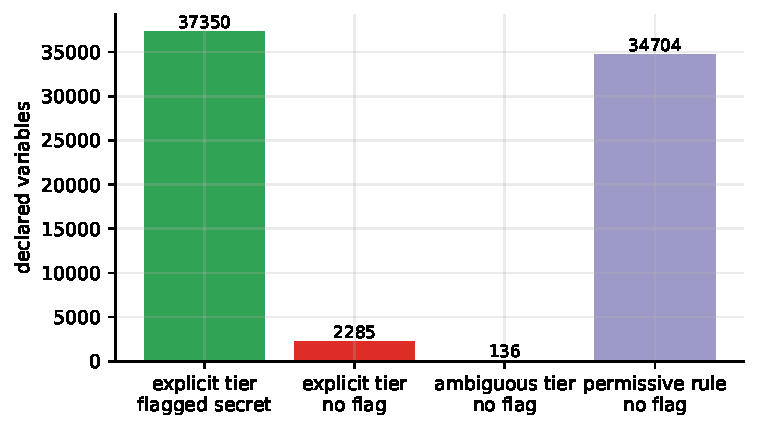
\includegraphics[width=\linewidth]{Figure_1}
\caption{Credential-like environment variables, split by whether the manifest
flags them secret. A client cannot redact automatically what the manifest does
not mark. Source: \texttt{t11\_credential\_hygiene.csv}.}
\label{fig:credential}
\end{figure}

Across the population the manifests declare 48,706 remote endpoints on 14,903
distinct hosts. Against expectation we found \textbf{no plaintext
\texttt{http} endpoints, no localhost endpoints, and a single endpoint on a
bare IP address}. This is a negative result that we attribute to the
registry's own validation rather than to publisher discipline
(\S\ref{sec:threats}), and we report it as evidence about the gatekeeper rather
than about the ecosystem.

Table~\ref{tab:rq2} reports the coding of 150 servers stratified by transport
(84 remote-only, 57 package-only, 7 both, 2 neither). Authentication could be
determined for 64.0\% of servers and remained undetermined for 36.0\%, a result
about artefact completeness as much as about security.

Two patterns matter. First, a substantial minority require no authentication at
all (52 servers, 34.7\%), consistent with read-only public data services.
Second, capability and scope concentrate: 51 servers expose at least one
writing tool and 10 a destructive one, 47 have broad scope, and \textbf{33
servers, 22.0\%, combine broad scope with write capability}, the combination
that turns a confused or compromised agent into a consequential event. Seven
servers gate access through payment rails (\texttt{x402} or prepaid credit)
rather than identity, a category we did not anticipate when writing the
codebook.

\begin{table}[t]
\caption{Security posture, coded by hand over 150 servers stratified by
transport.}
\label{tab:rq2}
\centering
\begin{tabular}{@{}lr@{}}
\toprule
Property & Servers (of 150) \\
\midrule
Authentication mechanism identified & 96 (64.0\%) \\
Authentication mechanism undetermined & 54 (36.0\%) \\
No authentication required & 52 (34.7\%) \\
Credential-based authentication & 37 \\
Payment-gated (x402, prepaid credit) & 7 \\
Requires the user to supply a secret & 24 \\
\quad of those, secret not flagged & 3 \\
At least one writing tool & 51 \\
At least one destructive tool & 10 \\
Broad scope & 47 \\
Broad scope and write capability & 33 (22.0\%) \\
\bottomrule
\end{tabular}
\end{table}

\subsection{RQ3: Evolution}

Growth was steep across the twelve months in the snapshot: from 787 published
versions in September 2025 to \textbf{27,863 in September 2026}, with
9,421 servers appearing for the first time in that final month alone.
Cumulative servers reached 35,388, and the curve shows no inflection
(Fig.~\ref{fig:growth}).

\begin{figure*}[t]
\centering
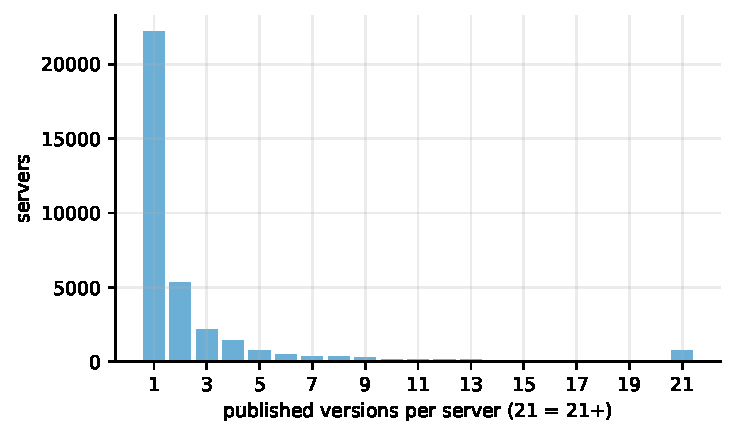
\includegraphics[width=\textwidth]{Figure_2}
\caption{Ecosystem growth over the twelve months of the snapshot. Bars give new
versions published per month; the line gives cumulative distinct servers. Both
are registry counts, so they measure publication rather than deployment.
Source: \texttt{t07\_publishing\_timeline.csv}.}
\label{fig:growth}
\end{figure*}

Growth is not distributed evenly. Table~\ref{tab:concentration} shows that the
100 most prolific namespaces, 0.49\% of the 20,540 namespaces, produce
\textbf{30.1\% of all published versions}, while the bottom half produce 9.0\%.
A single namespace published 2,387 versions, 2.1\% of the population by itself.
``Versions published'' is the most convenient proxy for activity in a registry,
and here it is dominated by a small number of automated publishers. Every
activity statistic in this paper therefore carries a median beside its mean,
and we state the concentration wherever a total appears.

\begin{table}[t]
\caption{Concentration of publishing activity across namespaces.}
\label{tab:concentration}
\centering
\begin{tabular}{@{}lr@{}}
\toprule
Namespaces & Share of versions \\
\midrule
Top 1 & 2.1\% \\
Top 5 & 8.4\% \\
Top 10 & 13.2\% \\
Top 25 & 18.8\% \\
Top 50 & 24.0\% \\
Top 100 & 30.1\% \\
Bottom 50\% (10,270) & 9.0\% \\
\bottomrule
\end{tabular}
\end{table}

\textbf{62.7\% of servers published exactly one version and never updated
again}, a further 16.1\% last published within 30 days of the freeze, and only
0.2\% had gone more than a year between their last two publications. 374
servers (1.1\%) are formally deprecated. Fig.~\ref{fig:churn} shows how
concentrated the release distribution is.

\begin{figure}[H]
\centering
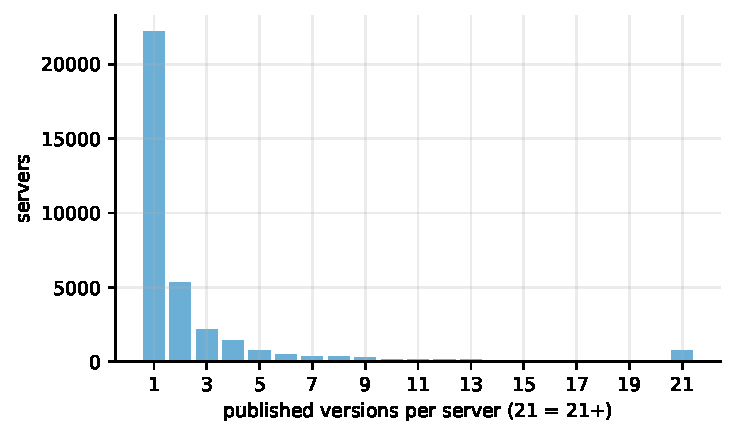
\includegraphics[width=\linewidth]{Figure_3}
\caption{Published versions per server. The distribution is dominated by
single-release servers, which is why every activity statistic in this paper
carries a median beside its mean. Source: \texttt{t08\_versions\_per\_server.csv}.}
\label{fig:churn}
\end{figure}

Package-based servers behave differently from hosted ones. Servers shipping an
installable package average 5.19 versions against 1.77 for hosted-only servers,
and declaring a repository is associated with 3.59 against 2.09. Deprecation
follows the same split: 1.8\% for package-based servers against 0.5\% for
hosted-only. The pattern is consistent with packages being versioned artefacts
and hosted endpoints being deployed in place.

Transports shifted during the window. Counting versions, the local
\texttt{stdio} transport still dominates at 67.0\%, but the hosted
\texttt{streamable-http} transport appears in 42.1\% of versions across 21,208
servers, more than \texttt{stdio}'s 15,009; hosted servers therefore publish
fewer versions each. The legacy \texttt{sse} transport is
residual at 2.4\%.

Packaging concentrates on npm (54.5\% of package declarations), then PyPI
(24.2\%), the MCP bundle format (10.9\%) and OCI images (9.1\%). Manifest schema
adoption is near-complete: 92.3\% of versions declare the 2025-12-11 schema.

Quality signals around those packages are weaker. Of 9,557 enriched npm
packages, \textbf{30.1\% declare no licence}, 67.4\% have a single maintainer,
2.1\% are deprecated, and 15.5\% recorded no downloads in the last month
(median 254). PyPI is worse on licensing: \textbf{85.0\% of 3,759 PyPI packages
declare no licence}, with 1.1\% carrying yanked releases.

Repository health points the same way. Of 751 resolved repositories, 20.4\%
declare no licence, 51.7\% have no stars and only 2.8\% have 100 or more, 5.6\%
have not been pushed in 180 days, and the median repository is 114 days old.
This ecosystem is young, distributed and almost entirely unstarred.

\subsection{RQ4: Inspectability}\label{sec:rq4}

Table~\ref{tab:completeness} reports field completeness across all 35,388
servers. Description and version are always present because the registry
requires them. Everything that would let an auditor act is optional:
\textbf{23.3\% of servers link no repository}, 39.2\% declare no remote
endpoint, 57.1\% declare no package and 50.9\% give no website. A quarter of
the population cannot be traced to source code at all.

\begin{table}[t]
\caption{Manifest field completeness across all 35,388 published servers.}
\label{tab:completeness}
\centering
\begin{tabular}{@{}lrr@{}}
\toprule
Field & Present & Missing \\
\midrule
description & 35,388 & 0 \\
version & 35,388 & 0 \\
repository & 27,146 & 8,242 \\
title & 21,767 & 13,621 \\
remotes & 21,526 & 13,862 \\
websiteUrl & 17,386 & 18,002 \\
packages & 15,166 & 20,222 \\
\bottomrule
\end{tabular}
\end{table}

Our pipeline reads as much as an automated reader reasonably can: it downloads
published package sources and parses the registration idioms of both official
SDKs. It
parsed 97.4\% of the sampled packages and recovered tools from 56.2\%. The
complement, 43.8\% of packages yielding no tool definition, is the
inspectability gap. Human validation on 150 packages (Table~\ref{tab:rq4})
shows the gap decomposes into two unequal parts: 69 of the 150 are not
tool-exposing servers at all, and only a small residue is genuine extraction
failure.

Where the pipeline did find a server it found essentially all of it:
\textbf{99.7\% recall and 99.7\% precision} on 1,794 hand-counted tools, with
five tools missed across two packages and five non-tools over-counted across
three. Every miss and every false positive falls in a Python package, where
pattern-based extraction of decorator-registered tools is weakest. We take this
seriously enough to have tried the obvious remedy: switching Python to an
AST-based extractor. Re-scoring against the same human ground truth showed
recall falling to 95.3\%, because the two readers have complementary blind
spots rather than one dominating the other. The validated configuration is the
one reported here.

\begin{table}[t]
\caption{Human validation of tool extraction over 150 packages.}
\label{tab:rq4}
\centering
\begin{tabular}{@{}lr@{}}
\toprule
Metric & Value \\
\midrule
Packages classified as a server & 81 \\
Servers where the extractor found at least one tool & 78 \\
Package-level detection rate & 96.3\% \\
Tools counted by hand & 1,794 \\
Tools matched by the extractor & 1,789 \\
Estimated tool-level recall & 99.7\% \\
Estimated tool-level precision & 99.7\% \\
\bottomrule
\end{tabular}
\end{table}

\subsubsection{Reliability of the human coding}\label{sec:reliability}

Two coders independently coded the same 50 items under one shared codebook and
one shared evidence pack. Agreement is reported per field rather than pooled: a
pooled figure would hide which claims are safe to make.

\begin{table}[t]
\caption{Inter-rater agreement over 50 shared items coded under codebook v1.2.
`Description states when to use' is reported over the 20 items the codebook's
worked examples do not cover; over all 25 it reaches $\kappa=0.779$. `Secret
documented' is not a reliability figure: the pack shows the manifest rule's
verdict for every item, so both coders applied a lookup rather than exercising
judgement.}
\label{tab:kappa}
\centering
\begin{tabular}{@{}llrr@{}}
\toprule
Part & Field & Observed & $\kappa$ \\
\midrule
C & description states purpose & 1.00 & 1.000 \\
C & description names side effects & 1.00 & 1.000 \\
B & write capability & 0.98 & 0.969 \\
B & authentication mechanism & 0.98 & 0.965 \\
B & authentication evidence & 0.98 & 0.964 \\
B & requires a secret & 0.98 & 0.964 \\
C & confusable with a sibling & 0.98 & 0.960 \\
B & destructive capability & 0.90 & 0.841 \\
B & scope breadth & 0.84 & 0.761 \\
C & description explains inputs & 0.82 & 0.725 \\
C & description states when to use & 0.95 & 0.643 \\
\bottomrule
\end{tabular}
\end{table}

Three things are worth reading off the table. The two fields that ask what a
description \emph{contains} --- whether it states a purpose, whether it named an
effect --- reached complete agreement, because v1.2 reduced them to questions
about the text itself. The two that require a judgement about whether a
condition is \emph{sufficient} --- selection guidance and input explanation ---
are the lowest, at 0.643 and 0.725. And the manifest-only rule for secret
declaration turned a field that had failed at 0.229 into a mechanical lookup,
which is what that entry records.

The claim about selection guidance therefore stands as a point estimate. On the
full 200-tool sample the coder marked 23.0\% (95\% CI [17.5, 29.0]); in this
round the two coders marked 8\% and 12\% of their 25 shared tools and agreed on
19 of the 20 items outside the worked examples. The field is reliable enough to
report as a proportion, and the paper does so.

One caveat belongs in the record rather than in the table. Round 2 measured the
same fields under a defective instrument: the second coder's pack carried no
evidence, and two value sets were ambiguous. Round 3 is the first round in
which both coders worked from the same complete material, so the two rounds are
not a before-and-after of coder skill. They are a before-and-after of instrument
quality, which is why the codebook revisions are described in \S\ref{sec:coding}
rather than hidden here.

%% ===========================================================================
\section{Discussion}\label{sec:discussion}

\subsection{Where the MCP ecosystem sits against established ones}

Every number in Section~\ref{sec:results} describes a twelve-month-old
ecosystem, which makes "is this a lot?" impossible to answer from the numbers
alone. Placing them beside package ecosystems measured at comparable maturity
changes what several of them mean.

\textbf{Concentration is not unusual; the concentration mechanism is.} Decan et
al.\ compared dependency-network evolution across seven packaging ecosystems and
found that growth statistics conceal very different underlying dynamics
\citep{decan2019}. Our finding that 100 of 20,540 namespaces produce 30.1\% of
versions is consistent with the heavy tails they report, so the concentration
itself confirms the established picture rather than departing from it. What
differs is where the tail comes from. In npm and PyPI, high-volume publishers
are mature libraries with long dependency histories; here the top namespace is a
single publisher that produced 2,387 versions of an agent's tool set. The tail
is generated by automated republication of one interface, not by accumulated
engineering. The practical consequence is that version counts, which are a
workable activity proxy in the ecosystems Decan et al.\ studied, are weaker here
which is what \S\ref{sec:t1-test} goes on to test.

\textbf{Single-release abundance contradicts an assumption carried over from
package ecosystems.} That 62.7\% of servers publish exactly one version and
never update again sits badly beside the maintenance expectations the packaging
literature establishes. Abdalkareem et al.\ showed that npm and PyPI carry a
large volume of trivial packages, so registry size overstates capability
\citep{abdalkareem2020}; our result extends that observation from package
\emph{content} to package \emph{trajectory}. A trivial package at least gets
published once and is usually a dependency of something. A single-release MCP
server may never be installed by anyone, and the registry counts it exactly like
a maintained one. Replication studies of technical leverage find that relying on
small or inattentive maintainers carries a measurable security cost
\citep{samaana2025}; our 67.4\% single-maintainer share says that most of this
ecosystem is in precisely that position.

\textbf{Withdrawal is rarer than in a mature registry.} Li et al.\ found that
9.6\% of Cargo packages have at least one yanked release and that the proportion
kept rising \citep{li2023yanked}. In our snapshot, 2.1\% of npm packages are
deprecated and 1.1\% of PyPI packages carry a yanked release. Two readings are
available and we cannot separate them with cross-sectional data. Either
withdrawal is genuinely rarer at this maturity, or the ecosystem is young enough
that the releases which will need withdrawal have not been published yet. Li et
al.'s rising trend supports the second, and the distinction matters: it implies
the withdrawal rate is a lagging indicator and will rise, so a client cannot
currently use low withdrawal rates as evidence of stability.

\textbf{Documentation converges on the mechanical and stops there.} Meng et
al.\ observed that developers' use of API documentation varies in ways a design
strategy must accommodate, and proposed guidelines accordingly
\citep{meng2019apidoc}; Fan et al.\ documented that documentation routinely
omits the information needed to decide how to use an operation
\citep{fan2020apidoc}. Our results locate the omission precisely. Naming has
converged almost completely (86.5\% \texttt{snake\_case}, enforced reverse-DNS
names), and purpose statements are near-universal at 93.5\%. What is missing is
the judgement-bearing part: a condition for choosing the tool. This is a
\emph{sharper} version of the finding those works report, because it identifies
which documentation element disappears when an interface is consumed by a model
rather than read by a person. Hora et al.\ show that interfaces evolve faster
than their documentation \citep{hora2016apievolution}; our 93.5\% ambiguity rate
suggests that for agent-facing interfaces, evolution is not even required to
produce the mismatch.

\textbf{Credential exposure has no established baseline, so we give a
mechanical one.} No prior work measures credential declaration in a tool
registry. The nearest frame comes from the agent-security literature. Khan et
al.\ evaluate defences against indirect prompt injection in tool-using agents
and find that restricting the available tools lowers attack success but also
lowers benign utility \citep{khan2026promptinjection}. Whether that trade-off is
acceptable depends on knowing what the tools can reach, which is exactly the
information our RQ2 shows is not declared. Yagoubi et al.\ find that sensitive
data leaks through tool arguments, a pathway that output-only audits do not
inspect \citep{yagoubi2026agentleak}; a client cannot audit a pathway whose
inputs the manifest does not mark as sensitive. Our 34,704 unflagged
credential-like variables are therefore not a cosmetic documentation gap. They
are the reason two published defence strategies cannot be applied without
reading source.

\subsection{Enforcing the shape of a declaration is direct; enforcing the
practice behind it is not}\label{sec:t1-test}

Version counts are the obvious way to describe an ecosystem's health, and this
study used them throughout. We tested whether they mean what they appear to
mean, against an independent signal: the releases each repository tags on
GitHub, for the 914 servers in the repository sample whose metadata resolved.

These two signals do not measure the same thing. \textbf{59.3\% of those servers
never tag a release at all} while continuing to publish to the registry, so
their median tagged-release count is zero against a median of two registry
versions. Repository releases cannot serve as ground truth for the population.
For the minority that do tag releases the relationship inverts: release counts
exceed registry versions for 24.9\% of servers, and the registry understates
releases by two times or more for 18.3\%. Rank agreement is weak to moderate
throughout (Spearman 0.379).

We draw a boundary rather than a conclusion, and the boundary generalises. The
registry is usable for \emph{presence} questions, such as whether a server ships
updates at all and in which month it first appeared, but not for \emph{cadence}
questions. The sub-day median interval between registry versions is an ingestion
artefact of batch publishing, not a release rhythm, and we do not present it as
one.

This is one instance of a more general property, and it is the claim we would
like other registry designers to take from this paper:

\begin{quote}
A registry can enforce the \emph{shape} of a declaration directly, because shape
is checkable at the moment of submission. Enforcing the \emph{practice} behind
the declaration takes post-hoc mechanisms, since practice happens afterwards.
Those mechanisms exist, and they are more expensive and slower, so a registry
that enforces only shape should be read as making a choice rather than facing a
limit. The distance between the two is measurable, and measuring it is the first
thing a population study of a registry should do.
\end{quote}

The evidence here is unusually clean because the same entity enforces both
things at different strengths. The MCP registry enforces naming: no server in
35,388 omits the slash separator, none departs from a reverse-DNS namespace, and
none puts a space in the server segment. It enforces nothing about release
practice, and on that axis the registry and the repositories disagree for 89.1\%
of servers in the sample. The registry also declares credential semantics
without enforcing them: a publisher may mark a variable secret, and 19.9\% of
credential-like variables are left unmarked. Shape is a submission-time
property; practice and semantics are not, and the gap between them is where
every measurement error in this paper originates.

Two consequences follow for anyone building a registry of agent-facing
artefacts. First, aggregate activity metrics computed from a registry inherit
its blind spots, so a census should test at least one headline series against an
independent source before reporting trends, which is what \S\ref{sec:t1-test}
does here. Second, properties worth enforcing are exactly those that are
shape-like: presence of a repository link, presence of a licence, presence of a
flag. Properties requiring judgement, such as whether a capability is broad or
whether a description is sufficient, resist enforcement, and the next
subsection explains why.

\subsection{What the agreement pattern shows}\label{sec:reliability-pattern}

Table~\ref{tab:kappa} was intended as a reliability disclosure and turned into
the paper's most transferable result. The fields do not fail uniformly. They
divide cleanly by what the coder is asked to judge.

Fields that ask whether a feature is \emph{present} reached moderate agreement
or better: whether a description states a purpose (1.000), whether it named a
side effect (1.000), whether a server can write (0.969), which authentication
mechanism it uses (0.965), whether it requires a secret (0.964), whether a
server can destroy (0.841), how broad its scope is (0.761). Coders looking for
the same visible thing find it, and two readers converge.

Fields that ask whether something is \emph{absent, sufficient or implied}
collapse to the lowest values in the table: whether a description states when to
choose the tool (0.643) and whether it explains its inputs (0.725). These are
not harder to read. They are harder to
agree on, because each requires a coder to decide what the absence of a
statement means. Under round 2's codebook the two coders on selection guidance
marked 6 and 1 of the same 25 items; tightening the rule and adding adjudicated
examples moved them to 0.643, and the residual disagreements stay of the same
kind: whether a stated purpose implies a selection condition, or whether an
explicit condition, trigger or ordering rule is required.

That mechanism explains the ecosystem's own behaviour, and this is the part we
consider new. A registry can check a presence at submission; a publisher can
supply one cheaply. Both sides therefore converge on the properties that are
presence-like, which is why naming is near-uniform and purpose statements are
near-universal. Sufficiency has no such equilibrium. There is no submission-time
check for it, and no shared standard for it: our own coders, working from the
same rule and the same evidence, still agree least on exactly those fields. The
ecosystem is not under-documented because publishers are careless. It is
documented exactly to the depth that a registry can reward, and no further.

Three practical consequences follow. A study that reports a single pooled
$\kappa$ will average a reliable measurement with an unreliable one and learn
nothing about either; per-field reporting is not pedantry. A governance
proposal that requires publishers to document sufficiency will not converge,
because the requirement cannot be adjudicated. And the parts of an agent
interface that most affect whether a model selects the right tool are precisely
the parts that resist both enforcement and measurement. That is a statement
about the limits of documentation-based governance rather than about this
registry.

\subsection{How the two propositions could be tested elsewhere}

Both propositions were derived from one registry during its first year, so the
useful question is not whether they are attractive but what would count as
evidence against them. Each is stated below with the observation that would
falsify it and the data a follow-up would need. Neither test requires access we
did not have.

\textbf{P1: enforcement strength at submission does not predict agreement with
independent practice.} What would falsify it is a registry that enforces only
shape and whose version counts nevertheless track an independent release signal
closely. Running that test requires only what is already here: for any registry
with a published version history and a linked source repository, compute rank
agreement between the two, as in \S\ref{sec:t1-test}. A Spearman correlation
above roughly 0.8 would show that the gap we measured is a property of this
registry or of its age rather than of submission-time enforcement.

A stronger design compares registries. A useful version takes two catalogues
that differ in enforcement and are otherwise comparable, for example one that
verifies publisher identity and manifest fields at submission and one that does
not, and measures the same quantity in both. Chrome Web Store listings and
VS~Code Marketplace extensions are candidates: both publish version histories,
both link repositories, and both differ from the MCP registry in that they run
post-hoc review as well as submission-time checks. That difference is the point
of the design, because it separates the two clauses of P1. If post-hoc review
narrows the gap while submission-time checks do not, the proposition gains the
causal reading we have avoided giving it here.

\textbf{P2: coding agreement tracks whether a field asks about presence or about
sufficiency.} Here falsification would be a field set in which sufficiency
judgements reach the agreement that presence judgements reach. Again the test is
a replication, this time with the codebook itself: apply \S\ref{sec:coding}'s
fields to another catalogue of declared interfaces, code a sample with two
independent coders, and compare the per-field $\kappa$ ordering. Model cards on
Hugging~Face, extension manifests in the VS~Code Marketplace and plugin
descriptions in OpenAI's tool ecosystem are all candidates, and all publish the
same kinds of artefact: a name, a free-text description, a machine-readable
parameter specification, and an optional link to source.

That prediction is specific enough to fail. We expect purpose and input
declaration to reach moderate agreement or better and selection guidance to
stay below 0.40, in any of those catalogues, because the asymmetry we attribute
to enforcement is really about what a coder can decide without inference. If
selection guidance instead reaches substantial agreement elsewhere, the
explanation in \S\ref{sec:reliability-pattern} is wrong and the mechanism lies
in the MCP artefacts rather than in the coding task.

Three limitations of these designs should be stated, because they bound what a
positive result would mean. Registry enforcement strength is not a manipulable
variable, so a cross-registry comparison is observational and confounded by age,
audience and governance model. Coding agreement depends on the coder population
as well as the field, so a replication with different coders confounds the two
unless the same codebook and evidence-pack procedure are used, which is why both
ship with this paper. And neither test addresses the case that matters most for
practice: whether a client that reads only the declared artefacts makes better
tool choices than one that does not. That is an experiment on agents, not on
registries, and it is the natural next step.

\subsection{What would have to become machine-checkable}

Our results suggest a short list of properties that are consequential, cheap to
declare and currently absent or optional. Each already has a natural home in
the manifest; none requires a new protocol.

\begin{enumerate}
\item \textbf{A required secret flag on every credential-like variable.} A
client cannot redact what the manifest does not mark, and 19.9\% of declared
variables are in that position today.
\item \textbf{A declared capability class.} Whether a server writes, deletes or
spends, and tool definitions answer it, but no artefact a client can read
before installing states it. 22.0\% of coded servers combine broad scope with
write capability, and a client currently learns this only by reading code.
\item \textbf{A selection condition on tool descriptions.} Descriptions state
purpose 93.5\% of the time but a condition for choosing the tool only 23.0\%
of the time, in an ecosystem where 93.5\% of tools have a
confusable sibling.
\item \textbf{A reachability declaration for auditing.} 23.3\% of servers link
no repository. Making the absence explicit would let a client distinguish
``closed source'' from ``unfinished manifest''.
\end{enumerate}

\subsection{Implications for practice}

An engineer deciding today whether to install an MCP server can check three
things and no more: whether a package exists and is licensed (30.1\% of npm and
85.0\% of PyPI packages are not), how many versions have been published (with
the caveat above), and which environment variables a manifest declares and
whether it flags them secret. Everything else requires reading source: capability,
scope, and whether the description distinguishes one tool from another. For a
quarter of servers there is no source to read.

For a publisher the same list inverts into inexpensive improvements, and the
ambiguity result suggests the change of highest value is disambiguating
siblings rather than writing better prose.

%% ===========================================================================
\section{Threats to Validity}\label{sec:threats}

We follow the four-category scheme and mark which threats we tested rather than
merely stated.

\subsection{Construct validity}

\textbf{Registry timestamps are not release dates.} Tested, and reported in
\S\ref{sec:t1-test}. The registry records ingestion; 59.3\% of servers never
tag a release at all. We restrict timing claims to presence and rephrase every
cadence claim accordingly.

\textbf{Extraction coverage as a proxy for documentation quality.} A server
whose tools cannot be extracted may generate them at runtime or document them
elsewhere. Recall was established against human ground truth on 150 packages
and is reported beside every tool-level claim.

\textbf{Secret flagging is a publisher declaration.} A variable not marked
secret is not necessarily mishandled at runtime. Our claim is narrower and
exact: a client cannot \emph{automatically} redact what the manifest does not
mark.

\textbf{The input-schema figure is a lower bound.} Only 3.2\% of tools expose a
schema our parser recovers. Publishers often pass schemas as variables or
generate them at runtime, so this measures static readability rather than
absence.

\subsection{Internal validity}

\textbf{Registry-side validation filters.} Absence of plaintext, bare-IP and
localhost endpoints is partly a property of the registry's validation, not
of publisher discipline. We report it as evidence about the gatekeeper.

\textbf{Version-count concentration.} A handful of namespaces publish thousands
of versions, so outliers dominate means and totals. We report every mean beside
a median and quote the concentration table wherever activity is discussed.

\textbf{Codebook defects discovered during coding.} The first inter-rater round
produced near-zero agreement on every field. Investigation showed two causes:
the handoff to the second coder carried no evidence, and two fields had
defective value sets. We revised the codebook twice, rebuilt the evidence pack,
and ran a further round in which both coders worked from the same complete
material. Only that round is reported as reliability.

Two limits on it belong here. The pack supplies the manifest rule's verdict for
the secret-declaration field, so that entry measures rule application rather
than judgement; and five of the coded tools appear as worked examples in the
codebook, so the selection-guidance figure is computed over the 20 items those
examples do not cover. Both are stated in Table~\ref{tab:kappa} rather than
only here.

\textbf{Sampling drift.} Any study of this population contends with growth. We freeze
the harvest at one date, record its digest, and draw every sample from that
snapshot.

\subsection{External validity}

\textbf{One registry, one protocol version.} Coverage is one registry during
its first year, with 92.3\% of versions on a single manifest schema.
Findings may not transfer to other agent-tool conventions.

\textbf{Two package registries.} Tool extraction covers only npm and PyPI, and
only the 1,200-package sample. The 10.9\% of package declarations in the MCP
bundle format and the 9.1\% in OCI images are not covered.

\textbf{Rapid change.} The ecosystem is twelve months old at the freeze.
Conclusions are properties of the window analysed; the pipeline is built to be
re-run at a later freeze.

\subsection{Conclusion validity}

\textbf{Recall and precision are estimated from counts, not identities.} The
coder recorded how many tools each package exposes rather than naming them, so
we estimate matching as the per-package minimum of the two counts. That
estimate holds in aggregate but cannot detect a package that over- and
under-counts at the same time.

\textbf{Cross-source comparisons are descriptive.} We report no $p$-values; the
relationships in \S\ref{sec:results} are associations.

\subsection{Reproducibility}

Sources are mutable and packages can be unpublished. Raw responses are cached,
every generated table is written to disk, and a manifest of SHA-256 digests
covers the snapshot, the samples and the outputs.

%% ===========================================================================
\section{Conclusion}\label{sec:conclusion}

We measured the MCP server ecosystem at a single frozen point, from the registry
outward, and validated each automated step against human judgement. The
ecosystem is large and growing steeply: 114,604 published versions across
35,388 servers, with 27,863 versions in the final month alone. It is also
unevenly built. Most servers publish once and stop; 100 namespaces produce
30.1\% of all versions; 23.3\% of servers cannot be traced to source at all;
and 19.9\% of declared environment variables look like credentials without
being flagged as such.

The result we did not expect concerns how the ecosystem documents itself. Its
conventions have converged on the mechanical parts, namely one naming style,
one manifest schema and near-universal description coverage, and have left the
judgement-dependent parts behind. Descriptions say what tools do; they rarely
say when to choose one, and 93.5\% of tools have a sibling an agent could
confuse them with. Two human coders could only reach fair agreement about which
descriptions give selection guidance, which suggests the difficulty is not
writerly but conceptual, and it will not yield to asking publishers to write
more.

The practical consequence is a short agenda: make the secret flag mandatory,
declare a capability class, add a selection condition, and state honestly when
no source is available. None requires a protocol change. All four would move
the agent-tool layer from partly auditable to mostly auditable.

Two findings travel beyond this protocol. A census of a registry measures
publication rather than practice, and here the two disagree for 89.1\% of the
servers we could check, so any population study of a young registry should test
at least one headline series against an outside source before reporting a
trend. And an ecosystem documents itself to the depth its registry rewards:
fields that ask whether a property is present are cheap to supply and easy to
agree on, so they converge, while fields that ask whether something is
sufficient are neither, so they do not. Both statements are consequences of
measuring the artefacts rather than the systems they describe, and both extend
to any registry of agent-facing components.

%% ===========================================================================
\section*{CRediT authorship contribution statement}

\textbf{Junan Chen:} Conceptualization, Methodology, Software, Validation,
Formal analysis, Investigation, Data curation, Writing -- original draft,
Visualization.

\section*{Declaration of competing interest}

The author declares that he has no known competing financial interests or
personal relationships that could have appeared to influence the work reported
in this paper.

\section*{Funding}

This research did not receive any specific grant from funding agencies in the
public, commercial, or not-for-profit sectors.

\section*{Data availability}

The replication package is deposited in Science Data Bank under DOI
\href{https://doi.org/10.57760/sciencedb.013wx}{10.57760/sciencedb.013wx} and
cited in the reference list \citep{replicationpackage}. It contains the
collection and analysis pipeline, the seeded samples, the generated result
tables, the coding codebooks with their worksheets, and a manifest of SHA-256
digests covering every artefact. Running the pipeline regenerates all raw data
from the public sources listed in Table~\ref{tab:sources}. The raw registry
snapshot is not redistributed, because the upstream registry is its
authoritative copy; the manifest lets the snapshot used here be verified
against a fresh harvest.

\section*{Declaration of generative AI and AI-assisted technologies}

Generative AI tools were used to help write and refactor the collection and
analysis code, and to assist with language editing of the manuscript. The
author reviewed and verified all code, all generated tables and all text, and
takes full responsibility for the content.

\section*{Acknowledgements}

The author thanks the second coder, who contributed the independent coding
reported in Section~\ref{sec:reliability} under a codebook shared with the
author, and two colleagues who read an earlier draft.

\bibliographystyle{cas-model2-names}
\bibliography{mcp-refs}

\bio{}
Junan Chen is a researcher at the University of Electronic Science and
Technology of China. His work focuses on empirical software engineering for
agent-facing infrastructure, with an emphasis on measuring software ecosystems
from published artefacts and on making such measurement reproducible.
\endbio

\end{document}
